\documentclass[letterpaper]{article} % DO NOT CHANGE THIS
\usepackage[submission]{aaai2027}  % DO NOT CHANGE THIS
% The serif, sans-serif, and monospaced fonts are loaded automatically by
% aaai2027.sty (newtxtext, helvet, courier). DO NOT add \usepackage{times},
% \usepackage{helvet}, \usepackage{courier}, or any other font package.
\usepackage[hyphens]{url}  % DO NOT CHANGE THIS
\usepackage{graphicx} % DO NOT CHANGE THIS
\urlstyle{rm} % DO NOT CHANGE THIS
\def\UrlFont{\rm}  % DO NOT CHANGE THIS
\usepackage{natbib}  % DO NOT CHANGE THIS AND DO NOT ADD ANY OPTIONS TO IT
\usepackage{caption} % DO NOT CHANGE THIS AND DO NOT ADD ANY OPTIONS TO IT
\frenchspacing  % DO NOT CHANGE THIS
%
% These are recommended to typeset algorithms but not required. See the subsubsection on algorithms. Remove them if you don't have algorithms in your paper.
\usepackage{algorithm}
\usepackage{algorithmic}

%
% These are recommended to typeset listings but not required. See the subsubsection on listing. Remove this block if you don't have listings in your paper.
\usepackage{newfloat}
\usepackage{listings}
\DeclareCaptionStyle{ruled}{labelfont=normalfont,labelsep=colon,strut=off} % DO NOT CHANGE THIS
\lstset{%
	basicstyle={\footnotesize\ttfamily},% footnotesize acceptable for monospace
	numbers=left,numberstyle=\footnotesize,xleftmargin=2em,% show line numbers, remove this entire line if you don't want the numbers.
	aboveskip=0pt,belowskip=0pt,%
	showstringspaces=false,tabsize=2,breaklines=true}
\floatstyle{ruled}
\newfloat{listing}{tb}{lst}{}
\floatname{listing}{Listing}

%
% Recommended for better-looking tables
\usepackage{booktabs}

%
% Keep the \pdfinfo as shown here. There's no need
% for you to add the /Title and /Author tags.
\pdfinfo{
/TemplateVersion (2027.1)
}

% DISALLOWED PACKAGES
% \usepackage{authblk} -- This package is specifically forbidden
% \usepackage{balance} -- This package is specifically forbidden
% \usepackage{CJK} -- This package is specifically forbidden
% \usepackage{float} -- This package is specifically forbidden
% \usepackage{flushend} -- This package is specifically forbidden
% \usepackage{fullpage} -- This package is specifically forbidden
% \usepackage{geometry} -- This package is specifically forbidden
% \usepackage{hyperref} -- This package is specifically forbidden
% \usepackage{navigator} -- This package is specifically forbidden
% (or any other package that embeds links such as navigator or hyperref)
% \usepackage{indentfirst} -- This package is specifically forbidden
% \usepackage{layout} -- This package is specifically forbidden
% \usepackage{multicol} -- This package is specifically forbidden
% \usepackage{nameref} -- This package is specifically forbidden
% \usepackage{savetrees} -- This package is specifically forbidden
% \usepackage{setspace} -- This package is specifically forbidden
% \usepackage{stfloats} -- This package is specifically forbidden
% \usepackage{tabu} -- This package is specifically forbidden
% \usepackage{titlesec} -- This package is specifically forbidden
% \usepackage{tocbibind} -- This package is specifically forbidden
% \usepackage{ulem} -- This package is specifically forbidden
% \usepackage{wrapfig} -- This package is specifically forbidden
% DISALLOWED COMMANDS
% \nocopyright -- Your paper will not be published if you use this command
% \addtolength -- This command may not be used
% \balance -- This command may not be used
% \baselinestretch -- Your paper will not be published if you use this command
% \clearpage -- No page breaks of any kind may be used for the final version of your paper
% \columnsep -- This command may not be used
% \newpage -- No page breaks of any kind may be used for the final version of your paper
% \pagebreak -- No page breaks of any kind may be used for the final version of your paper
% \pagestyle -- This command may not be used
% \tiny -- This is not an acceptable font size.
% \vspace{- -- No negative value may be used in proximity of a caption, figure, table, section, subsection, subsubsection, or reference
% \vskip{- -- No negative value may be used to alter spacing above or below a caption, figure, table, section, subsection, subsubsection, or reference

\setcounter{secnumdepth}{0} %May be changed to 1 or 2 if section numbers are desired.

% The file aaai2027.sty is the style file for AAAI Press
% proceedings, working notes, and technical reports.
%

% Title

% Your title must be in mixed case, not sentence case.
% That means all verbs (including short verbs like be, is, using,and go),
% nouns, adverbs, adjectives should be capitalized, including both words in hyphenated terms, while
% articles, conjunctions, and prepositions are lower case unless they
% directly follow a colon or long dash
\title{SGDAgent: Hierarchical Spatio-Temporal Scene Graph-Driven Agent for Structured Long-form Video Understanding}
\author{
    Anonymous Submission
}
\affiliations{
}

%Example, Single Author, ->> remove \iffalse,\fi and place them surrounding AAAI title to use it
\iffalse
\title{My Publication Title --- Single Author}
\author {
    Author Name
}
\affiliations{
    Affiliation\\
    Affiliation Line 2\\
    name@example.com
}
\fi

\iffalse
%Example, Multiple Authors, ->> remove \iffalse,\fi and place them surrounding AAAI title to use it
\title{My Publication Title --- Multiple Authors}
\author {
    % Authors
    First Author Name\textsuperscript{\rm 1,\rm 2}\equalcontrib,
    Second Author Name\textsuperscript{\rm 2}\equalcontrib,
    Third Author Name\textsuperscript{\rm 1}\corresponding
}
\affiliations {
    % Affiliations
    \textsuperscript{\rm 1}Affiliation 1\\
    \textsuperscript{\rm 2}Affiliation 2\\
    firstAuthor@affiliation1.com, secondAuthor@affilation2.com, thirdAuthor@affiliation1.com
}
\fi


\begin{document}

\maketitle

\begin{abstract}

Long-form video understanding requires semantic analysis and reasoning over hour-scale videos, yet faces fundamental challenges: incomplete coverage from lossy sampling, imprecise reasoning over long-range spatio-temporal interactions that flat representations fail to capture, and imprecise localization of sparse evidence buried in background noise.
Recent agentic approaches build searchable caption databases for iterative querying, but the evidence space remains fundamentally unstructured—flat text and embeddings cannot represent entity-level semantics or support traceable retrieval.
We propose \textbf{S}cene \textbf{G}raph-\textbf{D}riven Agent (SGDAgent), which restructures long video understanding by converting open-ended caption search into structured candidate verification.
Concretely, we (i)~design a hierarchical spatio-temporal scene graph structure for fine-grained video semantics representation, (ii)~build a bottom-up construction pipeline to generate such scene graphs, and (iii)~design a scene graph-driven agent following a propose-verify-answer paradigm with graph-based retrieval tools to search video content in a structured way.
Experiments across four benchmarks demonstrate substantial improvements: SGDAgent achieves +18.2\,pp accuracy gain on LVBench with matched settings, and the structured graph index enables lighter backbones to match stronger baselines.
Agent trajectory analysis confirms the gains stem from restructuring search itself—converting open retrieval into graph-anchored candidate verification.
\end{abstract}

% Uncomment the following to link to your code, datasets, an extended version or similar.
% You must keep this block between (not within) the abstract and the main body of the paper.
% Make sure that you do not de-anonymize yourself with these links.
% \begin{links}
%     \link{Code}{https://aaai.org/example/code}
%     \link{Datasets}{https://aaai.org/example/datasets}
%     \link{Extended version}{https://aaai.org/example/extended-version}
% \end{links}

\section{Introduction}
\label{sec:intro}

% - Para 1: Long-video understanding challenges -

% - Para 2: Current approaches and their limitations -

Long-form video understanding requires semantic analysis and reasoning over hour-scale videos, posing three fundamental challenges: \emph{incomplete coverage} from lossy frame sampling, \emph{imprecise reasoning} over long-range spatio-temporal entity interactions that flat embeddings or text fail to capture, and \emph{imprecise localization} of brief or cross-segment evidence buried in background noise.
Recent agentic video reasoning approaches\cite{deepvideo2025,videoagent,drvideo2025} convert videos into caption-centric databases and let LLMs iteratively query them.
Yet \emph{the evidence space remains fundamentally unstructured}: flat text and visual embeddings cannot represent high-order spatio-temporal semantics or support traceable retrieval.
Advances in multi-round retrieval\cite{videoagent}, grounding-verification pipelines\cite{videomind}, and multi-granularity toolkits\cite{videoseek} improve \emph{how the agent searches} without restructuring \emph{what it searches over}.

% - Para 3: Scene graphs as structured representation -

Scene graph is a structured representation that encode visual entities and their spatio-temporal interactions as graph nodes and edges\cite{scenegraph1,tpt2023}.
It offers a natural solution by providing exactly the entity-level and relational grounding that flat representations lack.
This provides key advantages highly aligned with long-video understanding needs: lightweight semantic modeling through compact structured language, high-order semantic structural constraints that align with human cognitive logic to facilitate reasoning, and precise retrieval capabilities via graph search techniques\cite{scenegraph1,scenegraph2,qiu2025step}.
Some existing works\cite{fei2024videoofthought, videoagent, omagent2024, vagent2025, deepvideo2025, drvideo2025} have attempted to convert video frames into textual descriptions or simple structured representations, and to construct large model-based agent frameworks for visual reasoning.
However, two gaps prevent their direct application to long-form video QA\@.
First, existing methods focus on frame-level or segment-level local relations, lacking unified cross-scale hierarchical organization to capture both instantaneous details and cross-segment causal chains\cite{tpt2023,vagent2025}.
Second, to our knowledge, prior graph-aware or agentic systems do not use scene graphs as the \emph{primary retrieval index} for long-form video QA; instead, they either treat graphs as auxiliary signals or retain caption-centric search as the dominant evidence space\cite{vagent2025,videoagent,deepvideo2025}.

% - Para 4: Our method — representation + agent workflow -

In this work, we present the \textbf{S}cene \textbf{G}raph-\textbf{D}riven Agent (i.e., SGDAgent), a novel framework that fundamentally restructures long-form video understanding by transforming traditional open-ended caption-based search into structured, graph-guided candidate verification.
Specifically, our contributions are threefold: (i)~We devise a hierarchical spatio-temporal scene graph architecture that precisely encodes fine-grained video semantics across multiple temporal scales; (ii)~We develop a bottom-up offline pipeline to efficiently construct and index this multi-level scene graph, enabling comprehensive representation at the frame, segment, and global levels, unified by a shared entity registry; (iii)~We introduce a reasoning agent anchored in the propose-verify-answer paradigm, leveraging graph-driven retrieval tools to systematically explore and verify video content within a structured search space.
The proposed SGDAgent leverages a hierarchical scene graph index to efficiently propose, verify, and answer questions through a structured and interpretable candidate verification process, fundamentally enhancing precision and robustness in long-video understanding.

% - Para 5: Results -

These designs yield substantial and consistent gains across benchmarks.
Under strictly matched settings on LVBench\cite{lvbench}, SGDAgent raises end-to-end accuracy from 54.8\% to 73.0\% (+18.2\,pp), boosts the answer rate from 83.5\% to 98.4\%, and cuts the failed-to-terminate (FTT) rate from 16.5\% to 1.6\% compared with the caption-only baseline.
Across four benchmarks, SGDAgent with the lighter \texttt{o4-mini} backbone nearly matches DVD\cite{deepvideo2025} with the substantially stronger \texttt{o3} on both LVBench and LongVideoBench\cite{longvideobench2024}, demonstrating that the structured graph index compensates for weaker open-ended search capability.
When paired with the same \texttt{o3} backbone, SGDAgent further outperforms DVD on all three long-duration benchmarks.
Ablation and trajectory analyses confirm that the improvement stems from restructuring the search process itself-shifting from open retrieval to graph-anchored candidate verification-rather than from the graph directly producing answers.

% - Para 6: Contributions -

In summary, we contribute (i)~a \textbf{hierarchical spatio-temporal scene graph representation} comprising frame-, segment-, and event-level graphs unified by a shared entity registry, together with a bottom-up offline construction pipeline; (ii)~a \textbf{scene graph-driven agent} that follows a propose-verify-answer paradigm with graph-guided candidate proposal, visual verification, caption fallback, and uncertainty-aware control; and (iii)~\textbf{comprehensive evaluation} on four benchmarks, with matched-setting ablations confirming that gains stem from restructuring the search paradigm rather than from the graph directly answering queries.

\section{Related Work}
\label{sec:related}

\textbf{Long-video understanding.}
With the rapid development of vision foundation models\cite{radford2021CLIP,li2022GLIP} and multimodal large language models\cite{llava2023,video-llava2024,bai2025qwen3vl}, video understanding has achieved remarkable progress on short-clip benchmarks\cite{caba2015activitynet}.
Yet hour-scale videos expose three fundamental bottlenecks that persist across both paradigm classes.
\emph{Large temporal span}: long videos span tens of thousands of frames; under context-window constraints, methods either sample discontinuously\cite{deepvideo2025} or compress visual tokens\cite{wang2025adaretake}, incurring inevitable spatio-temporal detail loss that degrades evidence-seeking performance\cite{lvbench,longvideobench2024}.
\emph{Complex spatio-temporal interactions}: entities exhibit diverse long-range dependencies—spatial relations, state transitions, and causal chains—that natural-language transcriptions lack the structural constraints to capture precisely\cite{zhang2024simplellm}.
\emph{Sparse critical evidence}: key clues are buried in fleeting actions or cross-segment causal links, easily obscured by background noise; multi-step reasoning agents\cite{videoagent,omagent2024} progressively narrow the search from coarse to fine but operate in implicit black-box spaces with rigid, pre-fixed workflows.
Against this backdrop, existing methods fall into two classes.
The first extends context capacity through longer windows, token compression, or hierarchical representations\cite{gemini15,qwen,internvl,seed,radford2021CLIP,li2022GLIP,llava2023,video-llava2024,bai2025qwen3vl,longvu2025,shu2025video,apollo2025}, yet must still locate sparse evidence within compressed representations.
The second treats it as a retrieval problem, mining information through selective sampling or agentic search\cite{deepvideo2025,mrvideo,videoseek,zhang2024simplellm,videorag2025,videotree2025,drvideo2025,yang2025vca}.
SGDAgent restructures the \emph{evidence space itself}—extending captions with a structured scene graph index where retrieval becomes candidate proposal grounded in entities, relations, and temporal constraints.

\textbf{Scene graph representation.}
Scene graphs encode visual entities and their spatio-temporal interactions as graph nodes and edges\cite{xu2017scene,tpt2023}.
Traditional generation pipelines follow a detect-then-classify paradigm, building graphs in sequential detection and relation recognition stages\cite{xu2017scene,motifs2018}.
Recent advances leverage vision-language models for open-vocabulary scene graph generation\cite{frompixel2024,vs32023,hyperglm2025}, enabling broader applicability in open-world scenarios, though precisely capturing cross-segment entity associations and complex temporal dynamics remains challenging.
Beyond generation, scene graphs serve as a semantic carrier for cross-modal retrieval and structured multimodal reasoning\cite{scenegraph1,scenegraph2,qiu2025step}; their formal topological structure also enables tight coupling with first-order logic for neuro-symbolic reasoning\cite{neuro2020,cai2025naver}, yielding highly interpretable inference pipelines.
Scene graphs have shown value in cross-modal reasoning\cite{qiu2025step}, embodied intelligence, and video understanding\cite{fei2024videoofthought,vagent2025,videomultiagents2025}.
However, most prior work treats scene graphs as auxiliary information embedded in fixed pipelines, lacking adaptive reasoning mechanisms that fully exploit graph topology.
SGDAgent differs by elevating scene graphs to the primary retrieval index, using graph structure to propose candidates and guide verification rather than merely augmenting caption-based search.

\begin{figure*}[!tb]
  \centering
  \includegraphics[width=0.96\textwidth]{../paper/figures/Graph.pdf}
  \caption{Hierarchical scene graph representation and bottom-up
  construction pipeline.  (a)~Keyframes are sampled from the long video.
  (b)~A VLM generates frame-level scene graphs; entity alignment
  maintains identity consistency via a shared video-level entity
  registry.  (c)~The three-level representation: frame-level graphs
  capture per-keyframe entity-relation snapshots, segment-level graphs
  aggregate temporal interactions within sliding windows, and the global
  event graph organizes high-level event semantics with explicit event
  edges.}
  \label{fig:graph}
\end{figure*}

\textbf{Agentic video reasoning.}
A growing body of work models long-video understanding as an agentic reasoning problem.
Early efforts fed per-frame or per-clip visual tokens directly into large language models\cite{video-llava2024,videochat2025}, but context-window limits and quadratic computation cost confine them to short clips and cause severe semantic loss on hour-scale inputs.
LLoVi\cite{zhang2024simplellm} addresses this by converting each clip into a text description that an LLM reasons over jointly; VideoRAG\cite{videorag2025} introduces retrieval-augmented generation to pre-index video content and retrieve relevant segments at query time; VideoTree\cite{videotree2025} builds a query-adaptive hierarchical representation for long-video reasoning; and DrVideo\cite{drvideo2025} reformulates long-video understanding as document retrieval over progressively refined text memory.
The field then shifted to interactive agentic loops: VideoAgent\cite{videoagent} controls multi-round frame retrieval through an LLM-driven state-action-observation loop; DVD\cite{deepvideo2025} establishes agentic search over a multi-granularity video database via the ReAct paradigm\cite{react2022}; VideoSeek\cite{videoseek} designs a multi-granularity toolkit that mirrors human seeking behavior; VideoMind\cite{videomind} implements localize-verify-answer phases through specialized roles on a unified backbone; VCA\cite{yang2025vca} uses curiosity-driven tree exploration for long-video navigation; and VAgent\cite{vagent2025} introduces graph-structured representations for retrieval, though limited to frame- or segment-level local relations without cross-scale unification or adaptive reasoning.
Recent work also explores multi-agent frameworks\cite{omagent2024} and neuro-symbolic reasoning\cite{neuro2020,cai2025naver}, and end-to-end post-training of LLMs with agent trajectories has emerged as an important trend\cite{team2026kimi,zeng2026glm}.
These methods improve search strategy flexibility, yet all operate over flat captions or raw frames.
SGDAgent transforms the search space itself: rather than stronger query reformulation over captions, we use scene graphs to propose entity- and temporally-grounded candidates, then verify visually, converting open-ended search into structured candidate verification.
 
\section{Methodology}
\label{sec:method}

\begin{figure*}[!tb]
  \centering
  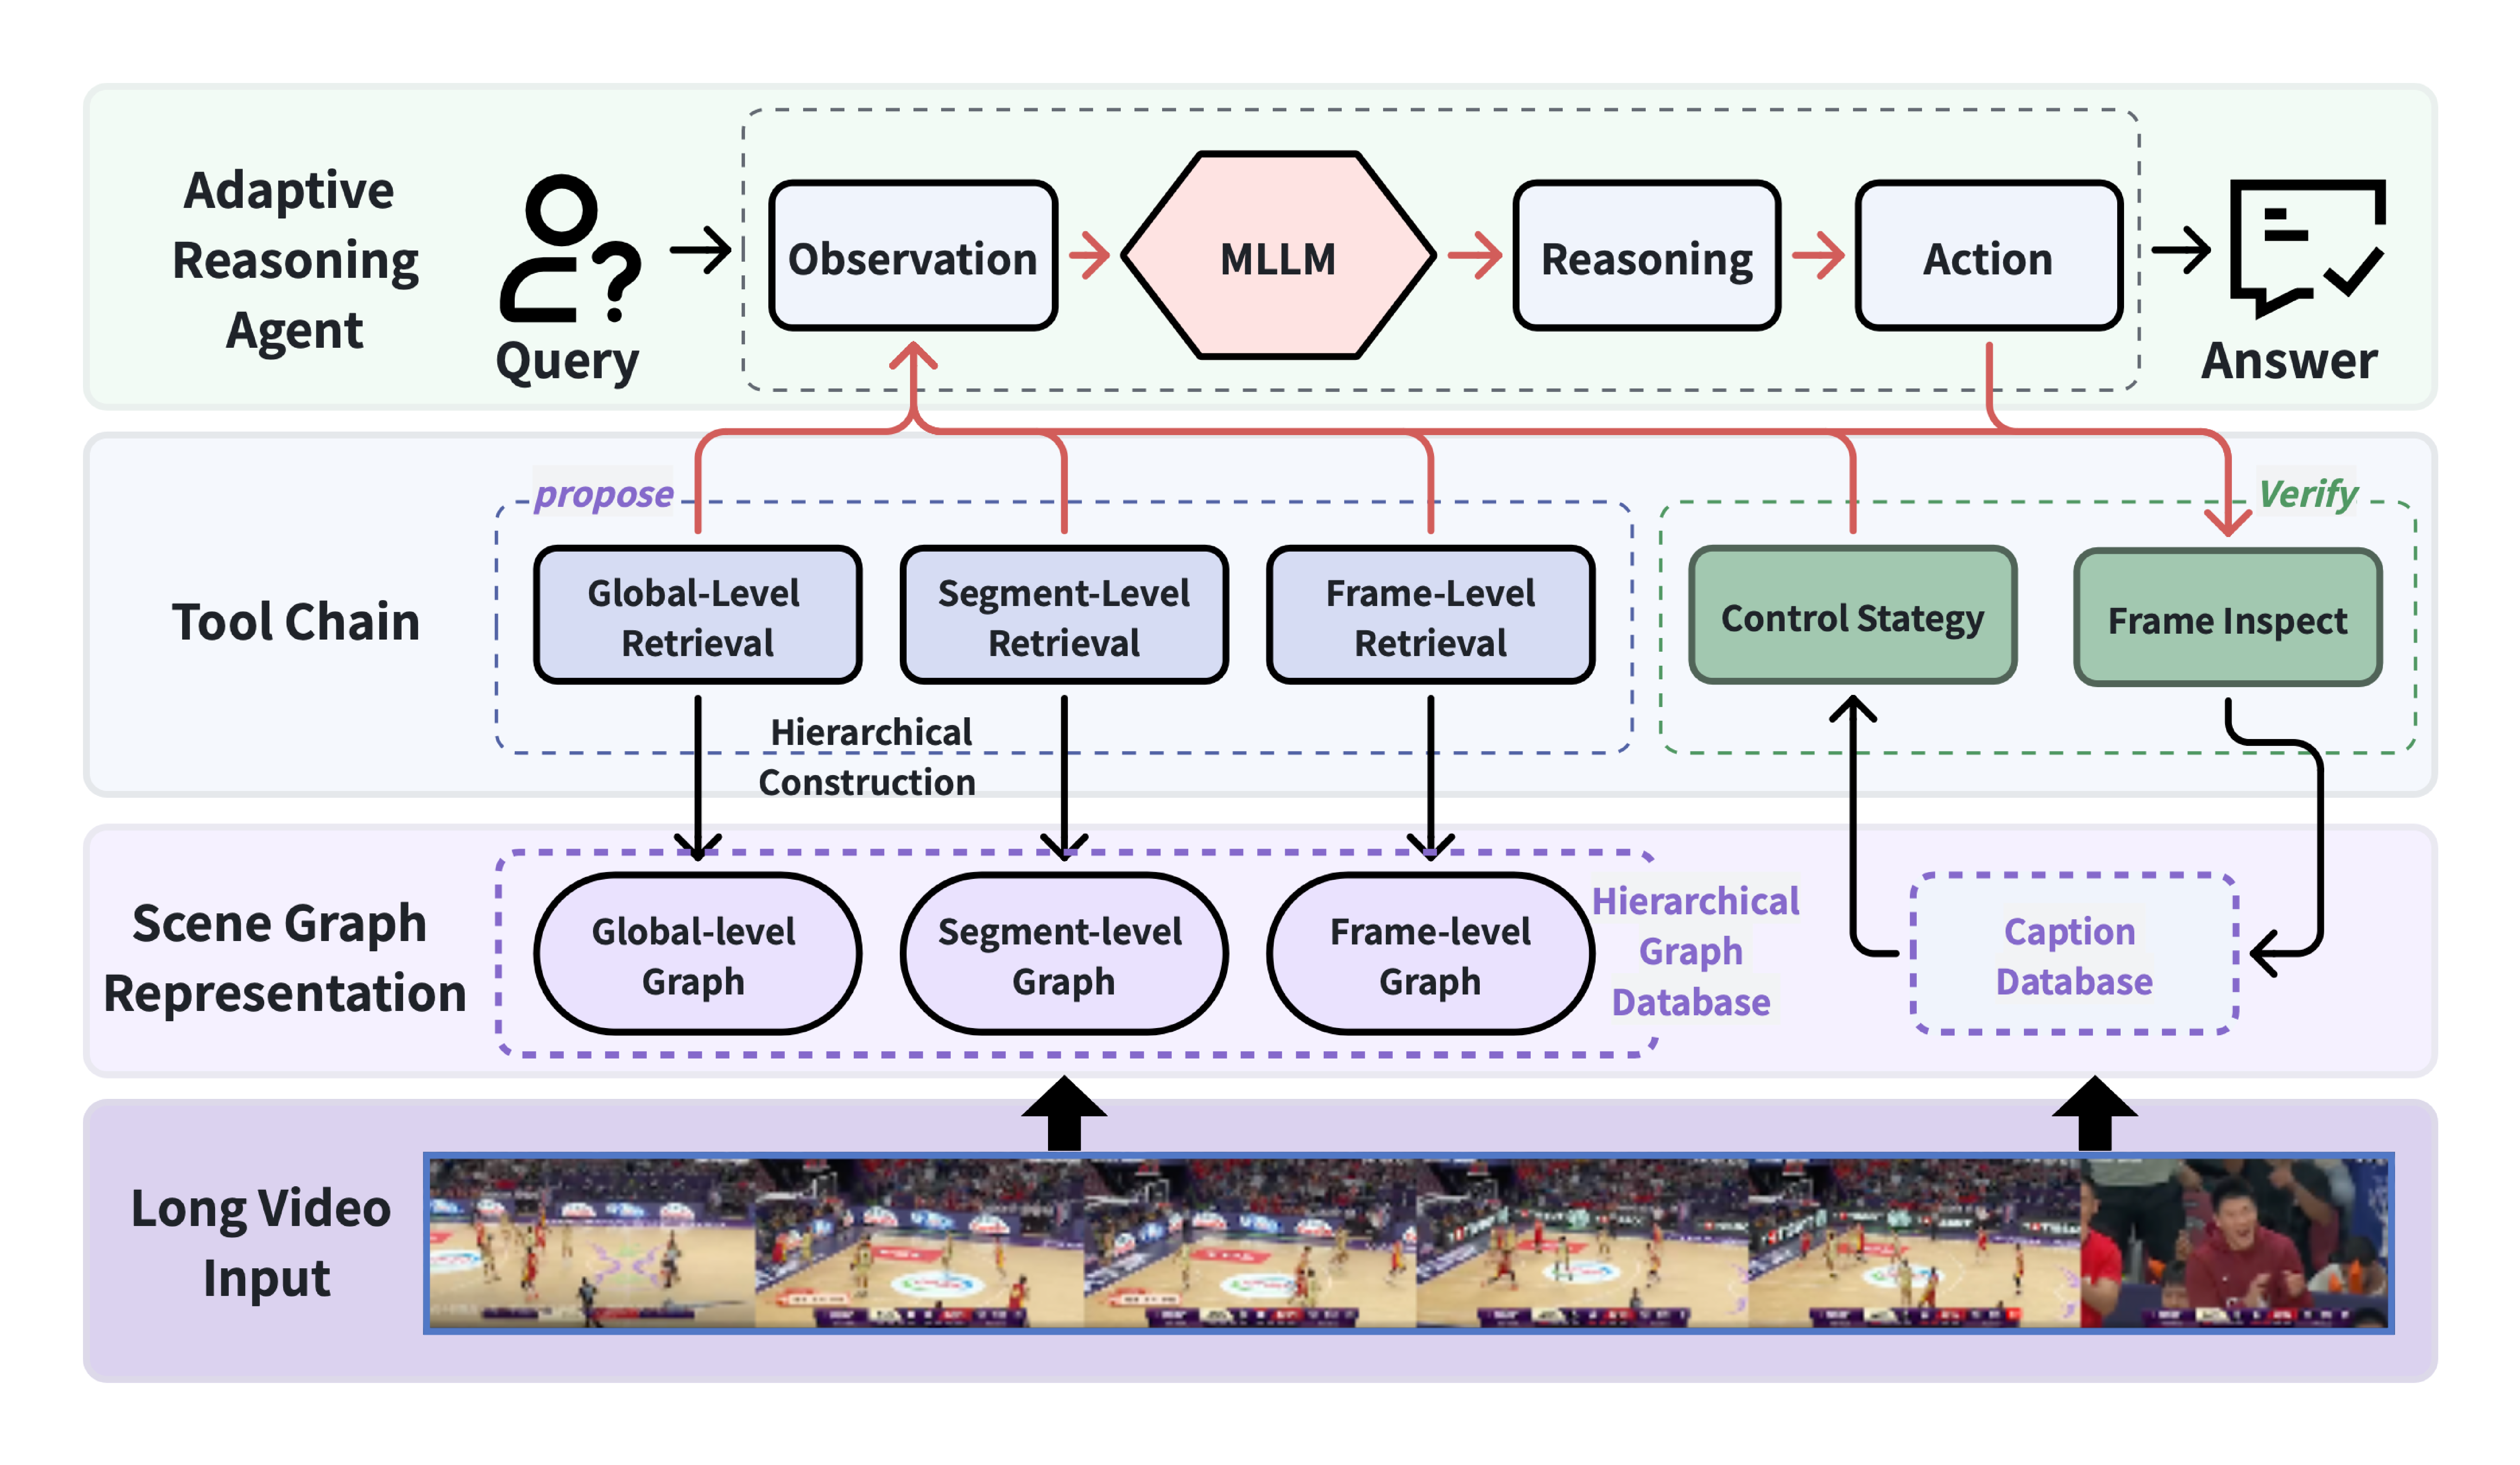
\includegraphics[width=0.96\textwidth]{../paper/figures/workflow.pdf}
  \caption{Scene graph-driven agent. Long videos are converted into a
  scene-graph-augmented video database with global-, segment-, and
  frame-level graphs plus a caption database. An adaptive reasoning
  agent then searches this database through a propose-verify tool
  chain within an observe-reason-act loop.}
  \label{fig:mechanism}
\end{figure*}


In this part, we introduce the \textbf{S}cene \textbf{G}raph-\textbf{D}riven Agent (SGDAgent), which uses a \emph{hierarchical scene graph representation} to index multi-granul video spatio-temporal semantics, and convert open-ended caption search into graph-anchored candidate verification.
Section \ref{sec:representation} first proposes the \textbf{hierarchical scene graph representation}, which builds the augmented video database $D(V)=\{C(V),\;G^{f},\;G^{s},\;G^{g}\}$.
Next, Section~\ref{sec:construction} introduces \textbf{bottom-up scene graph construction}, which extracts and aggregates the three graph levels offline; and Finally, Section~\ref{sec:agent} describe the proposed \textbf{scene graph-driven agent}, which runs an observe-reason-act loop under a \emph{propose-verify-answer} paradigm.

\subsection{Hierarchical Scene Graph Representation}
\label{sec:representation}

SGDAgent organizes video knowledge as caption database augmented with three-level spatio-temporal scene graph index (Figure~\ref{fig:graph} (c)):
\begin{equation}
  D(V) = \bigl\{C(V),\; G^{f},\; G^{s},\; G^{g}\bigr\},
\end{equation}
where $C(V)$ is caption database for open semantic retrieval; $G^{f}=\{G_i^{f}\}_{i=1}^{N}$ is frame-level graph sequence; $G^{s}=\{G_j^{s}\}_{j=1}^{M}$ is segment-level graph sequence; $G^{g}=(V^{g},\,\mathcal{E}^{g})$ is global event graph with event nodes $V^{g}$ and edges $\mathcal{E}^{g}$.
All three levels share video-level entity registry $E^{\mathrm{video}}$, where each entry stores unique ID, entity type, attributes, description, and temporal span (first and last appearance), serving as cross-scale identity anchor.

\textbf{Frame-level graph.}
Each frame-level graph captures entity-relation snapshot at single keyframe:
\begin{equation}
  G_i^{f} = (E_i^{f},\; R_i^{f},\; t_i,\; c_i),
\end{equation}
where $E_i^{f} \subseteq E^{\mathrm{video}}$ is visible entity set, $R_i^{f}$ is relation triples $(s, p, o)$ with $s,o \in E_i^{f}$ and predicate $p$, $t_i$ is timestamp, $c_i$ is aligned caption.
Frame-level graphs provide finest spatial granularity, anchoring objects and local relations to specific time points.

\textbf{Segment-level graph.}
Each segment-level graph aggregates entity interactions over short temporal window:
\begin{equation}
  G_j^{s} = (E_j^{s},\; R_j^{s},\;
  [t_j^{\mathrm{s}}, t_j^{\mathrm{e}}],\; F_j,\; s_j),
\end{equation}
where $E_j^{s}$ is active entity set, $R_j^{s}$ is temporal relations, $[t_j^{\mathrm{s}}, t_j^{\mathrm{e}}]$ is time range, $F_j$ is supporting frame IDs, $s_j$ is segment summary.
Each temporal relation is $(s, p, o, t_{\mathrm{start}}, t_{\mathrm{end}}, \mathcal{F})$, binding participants to temporal extent and supporting frames.

\textbf{Global event graph.}
Global event graph $G^{g}=(V^{g},\,\mathcal{E}^{g})$ organizes higher-level event semantics atop segments.
Each event node $n_k \in V^{g}$ is
\begin{equation}
  n_k = (P_k,\; R_k,\;
  [t_k^{\mathrm{s}}, t_k^{\mathrm{e}}],\; S_k,\; F_k,\; \sigma_k),
\end{equation}
where $P_k$ is participant entities, $R_k$ is salient relations, $[t_k^{\mathrm{s}}, t_k^{\mathrm{e}}]$ is event time range, $S_k$ is supporting segment IDs, $F_k$ is supporting frames, $\sigma_k$ is event summary.
Event nodes are typed as \emph{unit events} (compact episodes) or \emph{group events} (longer episodes).
Event edges $\mathcal{E}^{g}$ include \texttt{before}, \texttt{overlaps}, \texttt{entity-carryover}, \texttt{same-thread}, \texttt{parent-child}, encoding cross-segment chains and hierarchical structure.


\subsection{Bottom-up Scene Graph Construction}
\label{sec:construction}

We then develop a bottom-up pipeline to generate the hierarchical scene graph representation, as shown in Figure~\ref{fig:graph} (b).

\textbf{Frame graph extraction and entity alignment.}
Keyframes are uniformly sampled at fixed intervals.
For each keyframe, VLM produces structured scene graphs in single passes, outputting typed entities with attributes and relation triples.
Entity identity is maintained by greedily aligning each new entity to video-level registry $E^{\mathrm{video}}$ via weighted combination of name similarity, description similarity, type consistency; entities exceeding threshold $\tau$ merge, others register as new.
When VLM fails to extract entities, coarse-grained entities recover from temporally neighboring captions to prevent empty-graph gaps.

\textbf{Segment graph merging.}
Frame-level graphs aggregate into segment-level graphs via overlapping sliding windows.
Within each window, frame-level triples sharing $(s, p, o)$ signatures merge into single temporal relations spanning earliest to latest supporting frames; frame IDs and occurrence counts preserve.
Each segment graph includes textual summary; overlap links between adjacent windows support cross-boundary retrieval.

\textbf{Event graph construction.}
Temporally proximate and semantically coherent segments cluster into events.
Merging uses temporal gap, shared entity count, relation overlap, predicate overlap; overly long or discontinuous clusters split into unit events.
Group events form from multiple units via \texttt{parent-child} edges.
Pairwise edges—\texttt{before}, \texttt{overlaps}, \texttt{entity-carryover}, \texttt{same-thread}—infer from temporal ordering and entity sharing, completing event-level retrieval.

\textbf{Quality control.}
Lightweight constraints apply throughout: entity blacklist filtering removes generic entities, predicate whitelist suppresses noisy relations, schema validation enforces structural consistency.
At event level, confidence and uncertainty estimates attach to nodes for downstream gating.


\subsection{Scene Graph-Driven Agent}
\label{sec:agent}


\begin{algorithm}[!tb]
  \caption{SGDAgent: Graph-Driven Reasoning Loop}
  \label{alg:search}
  \begin{algorithmic}[1]
  % \small
  \REQUIRE Database $D(V)=\{C(V), G^f, G^s, G^g\}$, query $q$,
    budget $T$
  \ENSURE Answer $\hat{a}$
  \STATE $H \leftarrow \textsc{InitState}(q)$
    \COMMENT{routing state, candidates, evidence}
  \FOR{$t = 1, \ldots, T$}
      \STATE $a_t \leftarrow \textsc{LLM}(H)$
        \COMMENT{$a_t \in \{GR, SR, FR, FI, \textsc{Answer}\}$}
      \IF{$a_t \in \{GR, SR, FR\}$}
          \STATE $\mathcal{W} \leftarrow \textsc{QueryGraph}(a_t, q, D(V))$
          \IF{$\textsc{WeakSignal}(\mathcal{W}, H)$}
              \STATE $H \leftarrow \textsc{CaptionBackoff}(H, q, C(V))$
          \ELSE
              \STATE $H \leftarrow \textsc{UpdateCandidates}(H, \mathcal{W})$
          \ENDIF
      \ELSIF{$a_t = FI$}
          \STATE $e \leftarrow \textsc{FrameInspect}(\textsc{Top}(H), q)$
          \STATE $H \leftarrow \textsc{UpdateEvidence}(H, e)$
      \ELSIF{$a_t = \textsc{Answer} \land \textsc{GatingOK}(H)$}
          \STATE \RETURN $\textsc{Readout}(H)$
      \ELSE
          \STATE $H \leftarrow \textsc{RejectFinish}(H)$
      \ENDIF
  \ENDFOR
  \STATE \RETURN $\textsc{ForcedAnswer}(H)$
  \end{algorithmic}
  \end{algorithm}

Driven by the prebuilt hierarchical spatio-temporal scene graph to index multi-granul video semantics, a reasoning agent is designed as shown in Figure~\ref{fig:mechanism}.

\textbf{Adaptive reasoning agent loop.}
The agent operates in a closed loop following the observe-reason-act paradigm\cite{react2022} (Algorithm~\ref{alg:search}).
At each step~$t$, the agent \emph{observes} the current state~$H$, comprising the question, retrieved candidates, accumulated evidence, and control signals from prior tool calls.
The backbone LLM then \emph{reasons} over~$H$ and selects an action $a_t \in \mathcal{T}$.
The selected tool executes and its output—candidate windows, visual observations, or controller signals—updates~$H$ for the next iteration.
\textsc{Answer} is accepted only when accumulated evidence passes confidence gating; if the budget~$T$ exhausts without convergence, a forced readout extracts the best-supported option from the trajectory.

\begin{sloppypar}
\textbf{Tool chain.}\quad
% NOTE on GR vs.\ current implementation: the action set below reflects the
% target scene-graph architecture. In the present online system, a full GR
% over a true global scene graph is not yet realised as a callable tool; the
% global layer is approximated by (i) a Global Event Index---a prompt-injected
% timeline summary pre-computed from the segment-level graph---and (ii) a
% caption-based global-browse helper. Upgrading this to a tool-level query
% over a complete global scene graph is consistent with the hierarchy in
% Sec.~3.1 and is left as future work.
Following the propose--verify design of Figure~\ref{fig:mechanism}, the agent acts over $\mathcal{T}=\{GR,\,SR,\,FR,\,FI,\,CB,\,\textsc{Answer}\}$: three graph retrievers $\{GR,SR,FR\}$ propose candidate regions at progressively finer granularity, a pixel-inspection tool $FI$ verifies proposals against raw frames, and a caption backoff $CB$ supplies an orthogonal dense-text channel.
A distinctive feature of this tool chain is that every propose call returns not only ranked regions but also a vector of \emph{controller signals}---the retriever's own assessment of how far its output should be trusted---letting the agent assemble a self-aware cascade rather than a blind fusion of scores.

At the interface level the tool chain can be summarised as
\[
\begin{array}{rcl}
\textsc{GraphRetrieve}_{\ell}: & (q,\ \mathrm{scope},\ k) & \mapsto\ (\mathrm{regions}_{1:k},\ \mathrm{signals}), \\
\textsc{VerifyPixels}: & (\mathrm{window},\ q) & \mapsto\ \mathrm{evidence}, \\
\textsc{CaptionBackoff}: & (q) & \mapsto\ \mathrm{summary}.
\end{array}
\]
All three graph retrievers share a common scorer that ranks a candidate region $w$ against the query $q$ by
\begin{equation}
  S(w \mid q) \;=\; S_{\mathrm{lex}}(w,q) \;+\;
  S_{\mathrm{soft}}(w,q) \;+\; S_{\mathrm{temp}}(w,q),
\end{equation}
where $S_{\mathrm{lex}}$ aggregates token overlap scored \emph{separately} over entity names, relation predicates, and region summaries; $S_{\mathrm{soft}}$ is embedding cosine similarity where region vectors are available and degrades to lexical fuzzy match otherwise; and $S_{\mathrm{temp}}$ combines IoU with any time span parsed from $q$ and soft anchors inferred from cues such as \emph{beginning}, \emph{end}, or \emph{middle}.
A build-time entity blacklist further keeps video-production artefacts (``scene'', ``shot'', ``narrator'') and mis-extracted verbs out of both $S_{\mathrm{lex}}$ and $S_{\mathrm{soft}}$.
The $\mathrm{scope}$ argument carries a time constraint forwarded from a coarser-level call, and every returned region additionally carries a \emph{provenance pointer} to its supporting nodes at the next finer level---the scaffold on which the cascade is built.

\emph{Global-level retrieval.}\quad
$GR$ is the coarsest proposer and the natural entry point for video-spanning questions---causal, plot-level, or questions that arrive without any prior scope.
A call passes only the question, takes the entire video timeline as its search space, and returns a short list of event blocks spanning tens of seconds to minutes together with event-to-event relations (causal, temporal, co-participant) and provenance pointers down to the segments that support each event.
The agent consumes these outputs in two ways.
Each event's time span is forwarded as the $\mathrm{scope}$ of a subsequent $SR$ call, narrowing segment-level retrieval from whole- video to a few minutes in one step.
Independently, the event-to-event chain dictates the order in which events are visited when the question requires following a causal or temporal sequence, turning what would be a flat multi-hop search into a directed walk over the event graph.

\emph{Segment-level retrieval.}\quad
$SR$ is the primary proposer during online inference, invoked either cold or scoped by a prior $GR$ result.
It indexes sliding segments of roughly $10$--$30$ seconds, each aggregating entities and time-stamped temporal triples over a short window.
A call returns the ranked segment windows, the top temporal triples carried by those windows, provenance pointers to the supporting keyframes, and---crucially---the full controller-signal vector.
The agent uses $SR$'s time windows as the default input to $FI$ whenever pixel verification is warranted, and drills down through the provenance pointers to $FR$ when object- or relation-level grounding is needed.
Because $SR$'s output is structured, its controller signals can report quality along several axes at once: whether the top hit was only soft-matched, whether the best window is too wide for the question, and whether the question type demands visual detail the graph cannot settle on its own.

\emph{Frame-level retrieval.}\quad
$FR$ is the finest-grained proposer and is reserved for questions that need object-level grounding: specific attributes, identity, counts, or pairwise spatial relations at a particular moment.
It is invoked with a narrow $\mathrm{scope}$ forwarded from $SR$ and returns a ranked set of keyframes, each carrying an entity--attribute--relation snapshot anchored to a single timestamp.
Its output plays two roles.
The keyframe timestamps become the tightest possible inputs to $FI$, bounding pixel sampling to a window of a few seconds; and when the frame-level lexical evidence is strong and the snapshot alone answers the question, those entities and relations may be admitted as terminal evidence directly, bypassing pixel verification.

\emph{Pixel verification and caption backoff.}\quad
$FI$ is the only action that returns to raw pixels.
It consumes a graph-proposed time window, uniformly samples frames inside it, and runs a question-conditioned visual QA against those frames, producing terminal-grade visual evidence bound to a narrow, graph-localised region.
$CB$ instead queries an embedding-indexed caption database and returns a dense natural-language summary of matching clips; it covers the failure mode where the graph index lacks the surface form a question uses.
Both are terminal-capable but remain subject to the gating described next.

\emph{Controller-signal routing.}\quad
The controller signals emitted alongside every graph retrieval are the glue that turns the preceding interfaces into a coordinated cascade.
They summarise, in a form the agent can branch on, whether the top hit was lexical or fuzzy-only, whether the best region is too coarse for the question, whether the question demands a visual detail the graph cannot settle on its own, and whether the retriever recommends descending another level or escalating to pixel verification.
Three strategies consume them: \textbf{Strategy~R} (entry routing) maps question patterns such as counts, colours, or on-screen text directly to $FI$ without trusting any graph text, routes causal and plot-level questions from $GR$, and commits localisation questions to $SR$; \textbf{Strategy~G} (confidence gating) blocks \textsc{Answer} whenever a \emph{localize-only} or \emph{weak-match} signal is raised, escalates \emph{fine-detail}~plus~\emph{coarse-window} combinations to narrow-window pixel verification, redirects to $CB$ when graph evidence is weak but the question is not fine-detail, and enforces a finish gate that admits \textsc{Answer} only once the accumulated evidence is sufficiently narrow, targeted, and temporally valid; \textbf{Strategy~T} (terminal convergence) extracts the best-supported option from the accumulated trace once the budget $T$ is exhausted, preventing well-evidenced trajectories from degenerating into FTT outcomes.
The net effect is a coarse-to-fine cascade in which every hop is qualified by the retriever's own self-reported confidence rather than fused blindly into a single score---which we argue is the essential difference from single-signal RAG.
Section~\ref{sec:ablation} evaluates R, G, and T separately.
\end{sloppypar}


% ============================================================
%  Main Comparison Table — spans 4 benchmarks
% ============================================================

\begin{table*}[!tb]
  \centering
  \caption{Comparison on long video understanding benchmarks.
    LVBench\cite{lvbench} and Video-MME (Long)\cite{videomme2024} target hour-scale videos;
    LongVideoBench\cite{longvideobench2024} covers medium-to-long durations;
    EgoSchema\cite{egoschema2023} evaluates egocentric temporal reasoning over 3-minute clips.
    Methods are grouped by type: commercial VLMs, open-source VLMs,
    and video agents.}
  \label{tab:main_comparison}
  \small
  \begin{tabular}{ll cccc}
    \toprule
    & & \textbf{LVBench} & \textbf{LongVideoBench} & \textbf{Video-MME} & \textbf{EgoSchema} \\
    \textbf{Method} & \textbf{Backbone}
    & \textit{full}
    & \textit{Val, overall}
    & \textit{Long, w/o sub}
    & \textit{Val 500} \\
    \midrule
    \multicolumn{6}{l}{\textit{Commercial VLMs}} \\
    Gemini-1.5-Pro\cite{gemini15}
      & Gemini        & 33.1 & 64.0 & 58.6 & -   \\
    GPT-4o\cite{gpt4o}
      & GPT-4o        & 48.9 & 66.7 & 60.9 & 70.4 \\
    OpenAI o3\cite{o3}
      & o3            & 57.1 & 67.5 & 60.6 & 63.2 \\
    Gemini-2.5-Pro\cite{gemini25}
      & Gemini        & 67.4 & -   & -   & -   \\
    \midrule
    \multicolumn{6}{l}{\textit{Open-Source VLMs}} \\
    Qwen2.5-VL-72B\cite{qwen}
      & 72B           & 47.7 & 60.7 & -   & -   \\
    InternVL2.5-78B\cite{internvl}
      & 78B           & 43.6 & 63.6 & -   & -   \\
    Seed1.5-VL-Thinking\cite{seed}
      & Seed-VL       & 64.6 & -   & -   & -   \\
    \midrule
    \multicolumn{6}{l}{\textit{Video Agents}} \\
    VideoAgent\cite{videoagent}
      & -            & 29.3 & -   & -   & 63.2 \\
    MR.~Video\cite{mrvideo}
      & Gemini-Flash  & 60.8 & -   & 61.8 & 73.0 \\
    VideoMind\cite{videomind}
      & 7B            & 40.8 & -   & -   & -   \\
    VideoSeek\cite{videoseek}
      & GPT-5         & 68.4 & -   & -   & -   \\
    DVD\cite{deepvideo2025}
      & o4-mini       & 70.2 & -   & -   & -   \\
    DVD\cite{deepvideo2025}
      & o3            & 74.2 & 71.6 & 68.6 & \textbf{78.0} \\
    \midrule
    \multicolumn{6}{l}{\textit{Ours}} \\
    SGDAgent
      & o4-mini       & 73.0 & 71.2 & 65.1 & 73.9 \\
    SGDAgent
      & o3            & \textbf{75.9} & \textbf{74.0} & \textbf{69.0} & 77.4 \\
    \bottomrule
  \end{tabular}
\end{table*}

\section{Experiments}
\label{sec:experiments}

% ============================================================
%  Section 4.1  —  Experimental Setup
% ============================================================

\subsection{Experimental Setup}
\label{sec:setup}

\textbf{Dataset.}
Our primary benchmark is \textbf{LVBench}\cite{lvbench}, which contains 1{,}549 four-choice video QA questions over long-form videos.
The system receives a video, a natural-language question, and four candidate answers, and must return exactly one option; failure to do so is recorded as a failed-to-terminate (FTT) outcome.

\textbf{Implementation details.}
The reasoning backbone is \texttt{o4-mini} (temperature~0) with a maximum of 15 reasoning steps per question.
Frame-level scene graphs (Stage~1) are extracted by prompting \texttt{gpt-4.1} on keyframes sampled at one frame every 5~seconds (up to 120 per video).
Segment-level graphs (Stage~2) use 30-second sliding windows with 5-second overlap.
Local visual verification is performed by \texttt{gpt-4.1-mini}, with a budget of 50~frames per \texttt{frame\_inspect} call.
Graph retrieval returns at most 5 event-level, 6 segment-level, and 8 frame-level candidates.
To ensure fair matched-setting comparison, all internally compared methods share the same reasoning backbone, frame-inspect VLM, caption source, video database, candidate answer set, and budget limits; all methods are permitted to produce FTT outcomes.

\textbf{Evaluation metrics.}
We report four complementary metrics: \emph{end-to-end accuracy} (e2e\_acc), the fraction of all questions answered correctly; \emph{answered accuracy} (ans\_acc), accuracy computed only over questions for which the system produced a valid option; \emph{answer rate}, the fraction of questions that received a valid option; and \emph{FTT rate}, the fraction of questions where the system failed to commit an answer due to empty output, runtime failure, or trajectory non-convergence.


% ============================================================
%  Section 4.2  —  Main Results
% ============================================================

\subsection{Main Results}
\label{sec:results}

\textbf{Performance positioning.}
Table~\ref{tab:main_comparison} compares SGDAgent with published results across four long video understanding benchmarks.
Since these methods differ in backbone, caption source, and evaluation protocol, the numbers should be read as reference positions rather than controlled comparisons; the strict conclusions of this paper rest on the matched-setting ablations in Section~\ref{sec:ablation}.

Three observations are noteworthy.
First, \emph{the structured graph index narrows the gap between a weaker and a stronger reasoning backbone.}
SGDAgent with \texttt{o4-mini} achieves 73.0\% on LVBench\cite{lvbench} and 71.2\% on LongVideoBench\cite{longvideobench2024}, nearly matching DVD\cite{deepvideo2025} with the substantially stronger \texttt{o3} backbone (74.2\% and 71.6\%, respectively).
This suggests that when the evidence space is restructured from flat captions into entity-, relation-, and temporally-grounded candidates, the agent needs less raw reasoning power to locate the right evidence-the graph compensates for what the weaker backbone lacks in open-ended search capability.
Second, when paired with the same \texttt{o3} backbone, SGDAgent consistently outperforms DVD\cite{deepvideo2025} on the three benchmarks that emphasize long-duration and multi-entity reasoning (LVBench\cite{lvbench} 75.9 vs.\ 74.2, LongVideoBench\cite{longvideobench2024} 74.0 vs.\ 71.6, Video-MME Long\cite{videomme2024} 69.0 vs.\ 68.6), confirming that the gains from graph-guided candidate verification are additive to backbone strength rather than merely compensatory.
Third, on EgoSchema\cite{egoschema2023}-where videos are only 3~minutes and the graph hierarchy collapses to a handful of segments-SGDAgent (77.4) slightly trails DVD\cite{deepvideo2025} (78.0), consistent with the expectation that the structured proposal layer contributes most when the search space is large and evidence is temporally sparse.

\textbf{Matched-setting analysis.}
To isolate the contribution of each component under controlled conditions, Table~\ref{tab:main} reports matched-setting results on LVBench where all methods share the same backbone, caption source, and budget.

\begin{table}[!tb]
  \centering
  \caption{Matched-setting results on LVBench.
           All methods share the same backbone, caption source, and budget.}
  \label{tab:main}
  \begin{tabular*}{\columnwidth}{l@{\extracolsep{\fill}}cccc}
    \toprule
    Method & e2e\_acc & ans\_acc & ans rate & FTT rate \\
    \midrule
    Caption only          & 54.8\% & 65.7\% & 83.5\% & 16.5\% \\
    SG only               & 58.0\% & 69.1\% & 83.9\% & 16.1\% \\
    SGDAgent-base         & 64.4\% & 72.2\% & 89.2\% & 10.8\% \\
    SGDAgent (full)       & 73.0\% & 74.2\% & 98.4\% & 1.6\%  \\
    \bottomrule
  \end{tabular*}
\end{table}

\textbf{Effect of graph-augmented database.}
Combining the caption database with the scene graph index (SGDAgent-base) raises end-to-end accuracy by nearly 10 points over the caption-only baseline, while the full system with control strategies reaches 73.0\%.
Notably, using scene graphs alone (\emph{SG only}) is weaker than the combined configuration: its end-to-end accuracy exceeds caption-only by only 3 points, and its answered accuracy (69.1\%) still falls short of the combined configuration (72.2\%).
This confirms that the gain comes not from replacing captions with graphs, but from the complementary combination-the caption database preserves open semantic coverage while graphs contract the search space into verifiable candidate regions.
The following ablation study further dissects which graph levels and control strategies drive these gains.


% ============================================================
%  Section 4.3  —  Ablation Study
% ============================================================

\subsection{Ablation Study}
\label{sec:ablation}

Having established SGDAgent's overall effectiveness in Section~\ref{sec:results}, we now ablate its two core design dimensions under strictly matched settings: graph level depth (Sections~\ref{sec:representation}-\ref{sec:construction}) and agent control strategies (Section~\ref{sec:agent}).


% -----------
%  Experiment 1: Graph Levels
% -----------


\begin{table}[!tb]
  \centering
  \caption{Ablation on graph level depth. LLM calls and FI calls
           are per-question averages on full LVBench.}
  \label{tab:tiers}
  \begin{tabular*}{\columnwidth}{l@{\extracolsep{\fill}}cccc}
    \toprule
    Method & e2e\_acc & ans\_acc & LLM calls & FI calls \\
    \midrule
    Stage 1 only          & 59.2\% & 69.0\% & 4.92 & 2.38 \\
    Stage 1 + 2           & 64.6\% & 72.0\% & 10.3 & 5.34  \\
    Stage 1 + 2 + 3       & 64.4\% & 72.2\% & 2.94  & 1.35  \\
    \bottomrule
  \end{tabular*}
\end{table}

\textbf{Effect of graph level depth.}
Table~\ref{tab:tiers} dissects the contribution of each graph level.
The largest accuracy gain comes from adding the segment-level graph (Stage~1 $\to$ Stage~1+2), which provides the structured candidate discovery chain of ``frame-level localization + segment-level temporal organization.''
Adding the global event graph (Stage~3) does not further improve accuracy, but it cuts LLM calls by over $3\times$ (10.3$\to$2.94) and frame-inspection calls by $4\times$ (5.34$\to$1.35): event-level proposal narrows the search to relevant segments in one step, eliminating the need for exhaustive segment-by-segment exploration.
Stage~3 therefore contributes primarily as an efficiency layer rather than an accuracy layer.


% -----------
%  Experiment 2: Agent Control Strategies
% -----------


\begin{table}[!tb]
  \centering
  \caption{Effect of control strategies. SGDAgent-base uses the graph-augmented database with all three
           graph levels but no control strategies.}
  \label{tab:strategy}
  \begin{tabular}{lcccc}
    \toprule
    Method & e2e\_acc & ans\_acc & ans rate & FTT rate \\
    \midrule
    SGDAgent-base          & 64.4\% & 72.2\% & 89.2\% & 10.8\% \\
    + Strategy R           & 71.5\% & 78.0\% & 91.7\% & 8.30\%  \\
    + Strategy R + T           & 71.2\% & 72.1\% & 98.7\% & 1.30\% \\
    + Strategy R + G           & 70.2\% & 75.6\% & 91.0\% & 9.00\% \\
    + Strategy R + G + T       & 73.0\% & 74.2\% & 98.4\% & 1.60\%  \\
    ~~(= SGDAgent full)    &        &        &        &        \\
    \bottomrule
  \end{tabular}
\end{table}

\textbf{Effect of agent control strategies.}
Table~\ref{tab:strategy} evaluates the three control strategies introduced in Section~\ref{sec:agent}.
Strategy~R (query-type routing) improves answered accuracy from 72.2\% to 78.0\% while moderately reducing the FTT rate, indicating that it primarily raises answer quality by routing questions to appropriately targeted graph levels and visual verification.
Strategy~G (confidence gating) triggers caption backoff when graph evidence is weak; its standalone effect is modest, but it becomes essential in combination with Strategy~T, lifting end-to-end accuracy from 71.2\% (R+T) to 73.0\% (R+G+T) by providing more robust evidence before terminal readout.
Strategy~T (terminal convergence) addresses a different axis: it substantially compresses the FTT rate by recovering valid answers from trajectories that gathered sufficient evidence but failed to produce a well-formatted response.
The combination of all three strategies yields the best balance: end-to-end accuracy reaches 73.0\% with an FTT rate of only 1.6\%, confirming that routing improves \emph{how well} the agent answers, gating strengthens evidence coverage, and terminal convergence improves \emph{whether} it answers.

% -----------
%  Experiment 3: Efficiency
% -----------

\textbf{Efficiency analysis.}
Beyond accuracy, a central claim of this paper is that graph-anchored candidate verification restructures the search process itself.
Table~\ref{tab:behavior} compares per-question search cost between the caption-only baseline and SGDAgent variants across all questions with complete trajectory traces.
First, introducing segment-level graph retrieval (S1+2) substantially increases tool usage---LLM calls rise from 3.7 to 10.8 and frame inspections from 1.1 to 5.3---indicating that the accuracy gains come from deeper structured candidate discovery and stronger local verification, not from lightweight reranking of existing trajectories.
Second, adding the global event graph (full system) sharply reduces these costs while maintaining the accuracy gain: LLM calls drop from 10.8 to 3.4 ($3\times$) and frame inspections from 5.3 to 1.0 ($5\times$).
This confirms that the event-level proposal layer narrows search to relevant segments in fewer steps, serving as an effective efficiency mechanism on top of the accuracy-oriented segment-level graph.

\begin{table}[!tb]
  \centering
  \caption{Search efficiency comparison (per-question averages over
           questions with complete trajectory traces on LVBench).}
  \label{tab:behavior}
  \begin{tabular*}{\columnwidth}{l@{\extracolsep{\fill}}cccc}
    \toprule
    Method & ans\_acc & LLM calls & tool calls & FI calls \\
    \midrule
    Caption only      & 65.7\% & 3.69 & 3.53 & 1.10 \\
    SGDAgent S1+2     & 72.0\% & 10.8 & 10.3 & 5.34 \\
    SGDAgent (full)   & 74.2\% & 3.44 & 4.21 & 1.01 \\
    \bottomrule
  \end{tabular*}
\end{table}




% ============================================================
%  Section 4.4  —  Analysis on Agentic Reasoning Behavior
% ============================================================

\subsection{Analysis on Agentic Reasoning Behavior}
\label{sec:analysis}


\begin{figure*}[!tb]
  \centering
   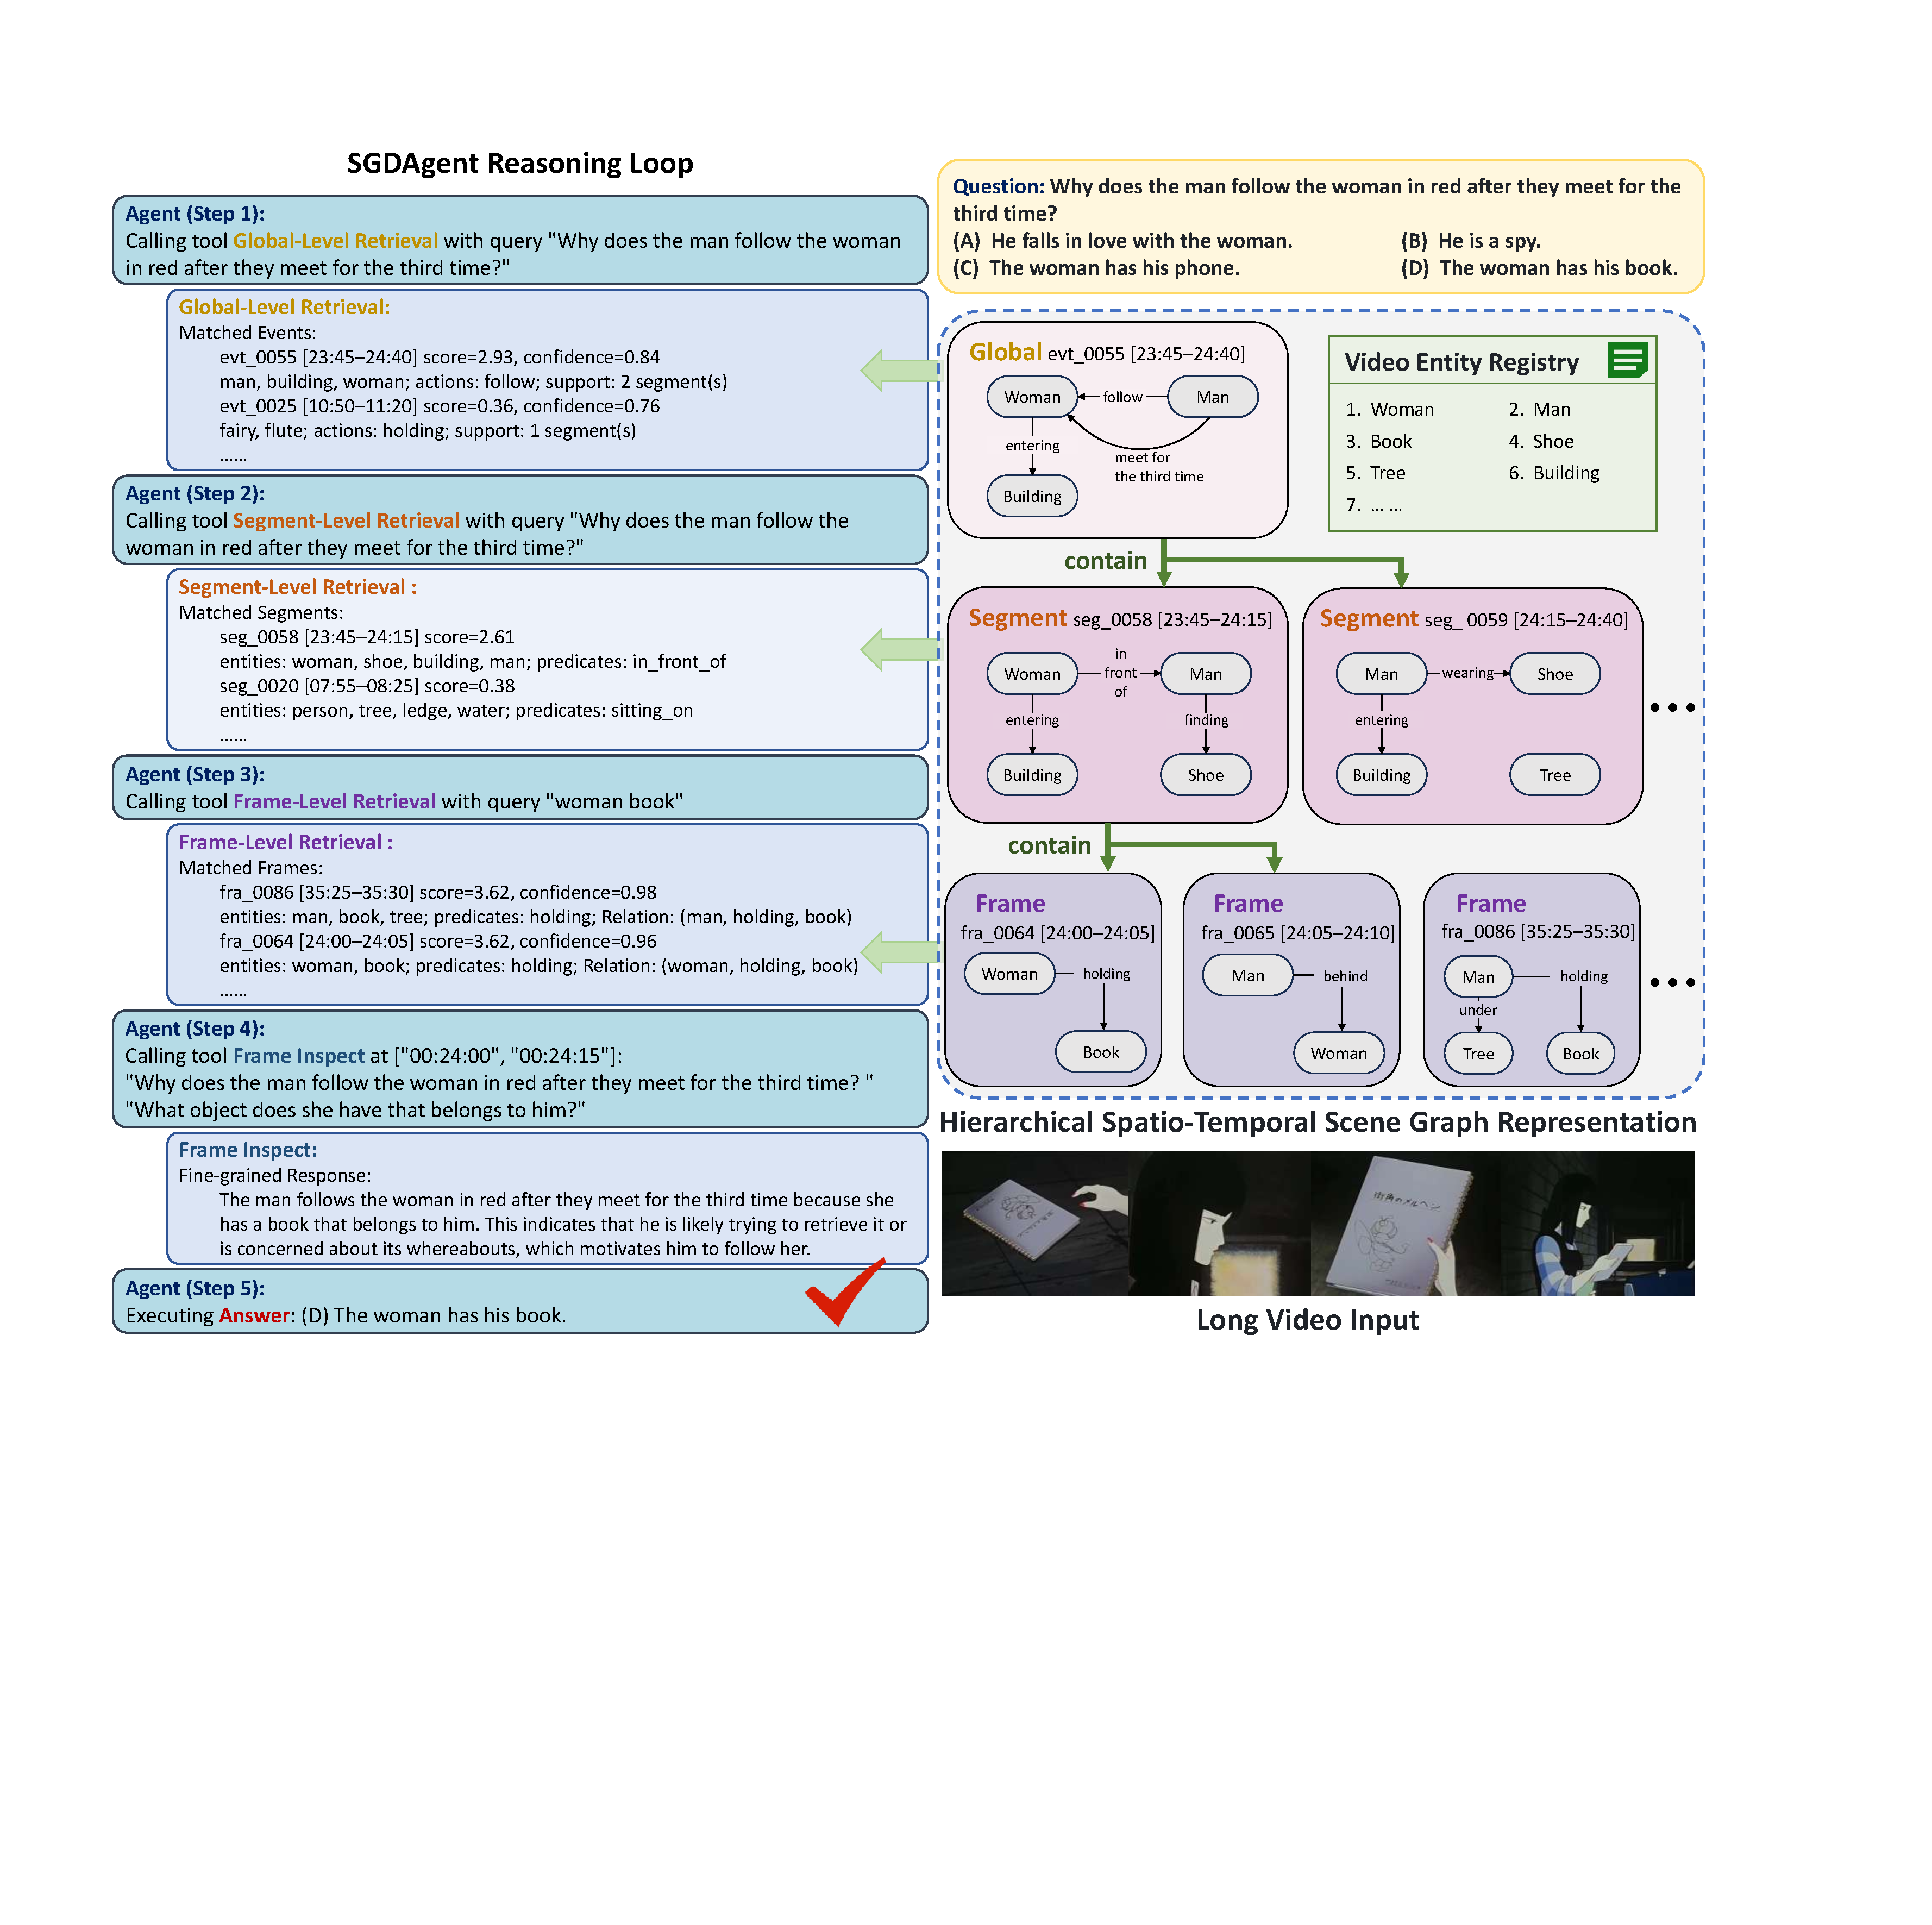
\includegraphics[width=\textwidth]{../paper/figures/Case.pdf}
  \caption{Case study from LVBench\cite{lvbench}, (qid: \texttt{q01CUy\_gwdU\_\_121}). SGDAgent reasoning trajectory on a motivational QA example: graph queries progressively narrow candidates from event to segment to frame level, guiding a single focused visual inspection to the correct answer.}
  \label{fig:trajectory}
\end{figure*}


The ablation results show \emph{what} improves; this section examines \emph{how} search behavior changes by comparing reasoning trajectories between the caption-only baseline and SGDAgent (Figure~\ref{fig:trajectory}).
The key finding is that graph-driven proposal replaces open-ended caption exploration with a focused cascaded narrowing, producing trajectories that are both shorter and more targeted.

\textbf{Case study: escaping the frame-inspect trap.}\quad
The question asks: ``Why does the man follow the woman in red after they meet for the third time?'' (correct answer: the woman has his book).
This is doubly challenging: the agent must first locate a specific \emph{repeated event} (the third encounter) within an hour-long video, then infer the \emph{motivation} behind the subsequent action by identifying a key object-possession relation.
The caption-only baseline follows $\mathrm{GB} \!\to\! \mathrm{FI}^{\times 5} \!\to\! \mathrm{Answer}$ and selects the wrong option.
Without structured intermediate representation, the agent cannot stably link ``the man,'' ``the woman in red,'' ``the third encounter,'' and ``the carried object'' into a coherent chain; it resorts to repeated broad-range frame inspections---each returning noisy local descriptions---until the budget is exhausted and an answer is forced from fragmentary evidence.
This is the \emph{frame-inspect trap}~\cite{deepvideo2025}.

SGDAgent follows $\mathrm{GR} \!\to\! \mathrm{SR} \!\to\! \mathrm{FR} \!\to\! \mathrm{FI} \!\to\! \mathrm{Answer}$, with each graph level progressively narrowing the candidate space.
$GR$ first anchors ``the third encounter'' to event \texttt{evt\_0055} [23:45--24:40] with high confidence, immediately reducing the search scope from the full video to a 55-second window with identified participants (woman, man) and the action ``follow.''
$SR$ localizes to segment \texttt{seg\_0058} [23:45--24:15], surfacing active entities (woman, man, building) and their spatial relations within the event window.
$FR$ queries ``woman book'' at frame level, retrieving \emph{person--holding--book} triples across keyframes (\texttt{fra\_0064}, \texttt{fra\_0086}), which provide direct entity-relation evidence for the candidate explanation.
A single focused $FI$ call on the narrowed window [24:00--24:15] confirms the book-possession relation and yields the correct answer.
In contrast, the baseline consumes five $FI$ calls spread across the entire video yet never assembles these cues into a coherent chain.

The graph does not directly answer the question but progressively compresses an open-ended ``why'' query into verification over a small candidate set: event anchoring narrows temporal scope, segment-level retrieval surfaces entity interactions, and frame-level triple matching provides object-relation evidence---each eliminating alternatives \emph{before} visual inspection begins.
This demonstrates that gains stem from restructuring search itself rather than from stronger frame inspection.


\section{Conclusion}

This paper presents SGDAgent, which restructures long-form video understanding by augmenting caption databases with hierarchical spatio-temporal scene graphs.
The core contribution is converting open-ended caption search into graph-anchored candidate verification through: (i)~a three-level scene graph representation (frame, segment, event) unified by shared entity registry; (ii)~a bottom-up construction pipeline; and (iii)~a graph-driven agent following propose-verify-answer paradigm.
Empirical results demonstrate that structured graph indexing fundamentally transforms search behavior.
On LVBench\cite{lvbench}, SGDAgent achieves +18.2\,pp accuracy gain with 98.4\% answer rate.
The structured index enables lighter backbones (\texttt{o4-mini}) to match stronger DVD baselines\cite{deepvideo2025} built on \texttt{o3}, confirming that graph-guided candidate verification compensates for weaker reasoning capability.
Ablations reveal segment-level graphs drive accuracy gains through structured candidate discovery, while event-level graphs provide efficiency through cascaded retrieval.
Trajectory analysis confirms improvements stem from restructuring search itself—not from graphs directly answering queries—by converting open retrieval into entity- and temporally-grounded candidate verification.


% %%
% %% Acknowledgments
% %%
% \begin{acks}
% % Hidden during anonymous review. Fill in after acceptance.
% \end{acks}

%%
%% Bibliography
%%
\bibliography{../paper/references}

\end{document}
